\documentclass[10pt,conference,compsocconf]{IEEEtran}
\usepackage{graphicx}
\usepackage{subfigure}
\usepackage{multirow}
\usepackage{balance}
\usepackage{blindtext}
\usepackage[justification=centering]{caption} %% for centering the caption
\usepackage[belowskip=-5pt,aboveskip=10pt]{caption} %for the blank above and below caption
% correct bad hyphenation here
\hyphenation{op-tical net-works semi-conduc-tor}


\begin{document}
%
% paper title
% can use linebreaks \\ within to get better formatting as desired
\title{Improving big data processing at large scale on supercomputers using multithreading and advanced MPI features }


% author names and affiliations
% use a multiple column layout for up to three different
% affiliations


\author{ \IEEEauthorblockN{Boyu Zhang\IEEEauthorrefmark{1}, Wesley 
    Bland\IEEEauthorrefmark{2}, Pavan Balaji\IEEEauthorrefmark{3},
    Michela Taufer\IEEEauthorrefmark{1}}
  \IEEEauthorblockA{\IEEEauthorrefmark{1}University of Delaware
    \\\{bzhang, taufer\}@udel.edu}
  \IEEEauthorblockA{\IEEEauthorrefmark{2}Intel Corporation
    \\wesley.bland@intel.com}
  \IEEEauthorblockA{\IEEEauthorrefmark{3}Argonne National Laboratory
     \\balaji@anl.gov} }

% make the title area
\maketitle

\begin{abstract}
%\boldmath
NA.
\end{abstract}

% IEEEtran.cls defaults to using nonbold math in the Abstract.
% This preserves the distinction between vectors and scalars. However,
% if the conference you are submitting to favors bold math in the abstract,
% then you can use LaTeX's standard command \boldmath at the very start
% of the abstract to achieve this. Many IEEE journals/conferences frown on
% math in the abstract anyway.

% no keywords
% For peer review papers, you can put extra information on the cover
% page as needed:
% \ifCLASSOPTIONpeerreview
% \begin{center} \bfseries EDICS Category: 3-BBND \end{center}
% \fi
%
% For peerreview papers, this IEEEtran command inserts a page break and
% creates the second title. It will be ignored for other modes.
\IEEEpeerreviewmaketitle



\section{Introduction}
\label{introduction}

The goal of this work is to bridge big data processing on HPC platforms 
such as supercomputers. MapReduce model provides an easy way for
application programmers to deal with distributed big data. Moreover,
there exist many runtime libraries that support MapReduce on cloud
environment such as hadoop etc. At the same time, HPC platforms such
as supercomputers provides high performance computation (multicore per node),
 communication (MPI), and storage capabilities (high performance shared
 file system such as lustre).

Some research effort targets to bridge big data processing
on HPC platforms such as supercomputers. This is important due to
the fact that many scientific applications (e.g. xx, yy) run on HPC platforms,
they generate big data that need to be processed in an in-situ or in-transit manner
(cite xx). MapReduce-MPI is a popular framework that enables big data
on HPC platforms. However, MRMPI has poor performance at large
scale. Figure xx shows for benchmark word count and clustering,
when using 2048 computing cores, the weak scalability is bad due to
the long shuffle time that involves all to all communications. The root
of the poor performance is two design choices: (1) MRMPI uses a process-based
model. Each MPI process runs map and reduce functions. To take advantage
of multiple computing cores per node, one needs to run multiple MPI
processes per node. This results in communication happens 
from process to process, hence multiple communication channels established
among two nodes which in fact only 1 is needed. (2) MRMPI uses blocking
MPI\_Alltoallv to do the all to all communication in the shuffling stage. This
precludes the possibility of overlapping communication and computation
in the process. These two design choices increase the number of
processes involved in the all to all communication, and block computation
while communication is undergoing. 

In our new design, we overcome these two disadvantages by using:
(1) a hybrid MPI process and multithreaded based model. Each MPI
process runs multithreaded version of map and reduce functions. One
can take advantage of multiple computing cores per node by running
one process on each node, and running multithreaded map and reduce
functions per node. This reduce the number of process involved in the
all to all communication, ensures that the communication happens 
among nodes, which is the minimum communication size; (2) non-blocking
MPI\_Ialltoallv communication which is available since MPI version xx.
This allows overlapping of communication with map computation.

The evaluation using benchmarks show that our new MapReduce
model improves the performance at large scale.

This paper makes three significant contributions:
\begin{itemize}
\item It presents a MapReduce runtime library using multithreaded 
design and advanced MPI features.
\item It improves the scalability of big data processing on supercomputers
at large scale.
\item It shows ...
\end{itemize}

The rest of this paper is organized as follows:
Section~\ref{s:related_work} reviews the related work on trajectory
analysis and distributed big data analytics; Section~\ref{s:method}
presents our method in detail; Section~\ref{s:validation} shows the
validation of the method using statistical and empirical techniques;
Section~\ref{s:implementation} discusses the implementation aspects in
Parallel MATLAB; Section~\ref{s:evaluation} presents the performance
evaluations; and Section~\ref{s:conclusions} concludes the paper and
gives directions for future work.

\section{Background}
\label{background}
\subsection{MapReduce and MapReduce-MPI}
MapReduce programming model. 
\begin{itemize}
\item map function, key value, run in parallel
\item shuffle, group all values with same key
\item reduce function, key value, run in parallel
\end{itemize}
MapReduce-MPI is a runtime library written in C++ and MPI that
enables MapReduce operations on HPC platforms.
\begin{itemize}
\item mrmpi runs map and reduce function in an individual process.
\item map, read input, apply map function, output intermediate 
output to disk files
\item communication, after map is done on all processes, 
mpi alltoallv
\item reduce, after communication is done, apply reduce.
\end{itemize}

\subsection{Non-blocking MPI collectives}
discuss the blocking MPI\_Alltoallv vs. non-blocking MPI\_Ialltoallv.


\section{The MTMR system}
MTMR implements MapReduce for traditional HPC systems such as 
supercomputers. Its goal is to enable efficient big data processing
at large scale.

\subsection{The MTMR API}
The current MTMR provides an application programming interface (API)
for C and C++. Similar APIs can be defined for other languages such as
Java. The API includes three main functions summaries in Table xx.

Map local xxx

Map xxxx

Reduce xxx.


\subsection{MTMR runtime design}
Key points:

\begin{itemize}
\item Push communication part of shuffle to map, push reorganization part of
shuffle to reduce.
\item Two techniques to gain performance: using multithreading to take advantage
of intra-node parallelism, and using nonblocking MPI collectives to overlap
communication and computation.
\end{itemize}

The MTMR is developed using C++, MPI, and OpenMP. It uses OpenMP to
enable multithreaded processing in map and reduce functions. It uses 
non-blocking MPI collectives to communicate $<$key, value$>$ pairs 
between map and reduce phases, and to overlap communication
with map computation. Figure~\ref{fig:overview_mtmr} shows the overall
design of MTMR runtime. 
\begin{figure}[!htb]
\centering
  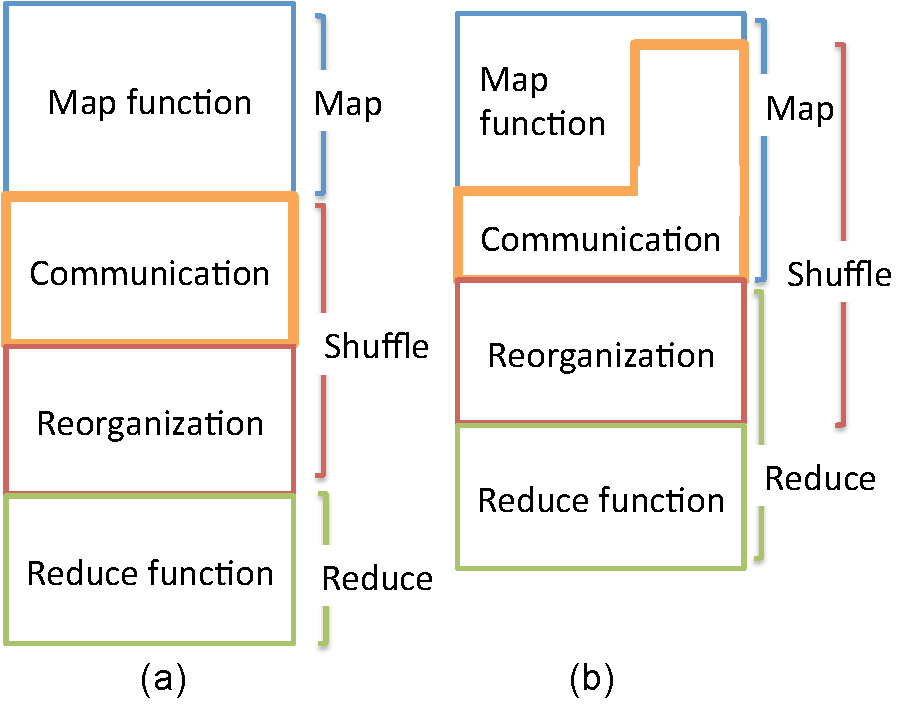
\includegraphics[width=0.9\linewidth,height=2.2in]{figs/overview_mtmr.pdf}
  \caption{MapReduce operations: map, shuffle, and reduce operations in a
  typical MapRedue runtime such as MapReduce-MPI (a); and map, shuffle, and
  reduce operations in our MTMR runtime (b).}
  \label{fig:overview_mtmr}
\end{figure}

In a typical MapReduce runtime library such as MapReduce-MPI, the library
implements three major phases: map, shuffle, and reduce, as shown in 
Figure~\ref{fig:overview_mtmr}(a). Map phase reads the initial input and
emits the intermediate $<$key, value$>$ pairs. Shuffle phase communicates
all the $<$key, value$>$ pairs with the same key to the same process
and forms the key and list of values as the input to reduce function. It
can be divided into two steps: communication and reorganization. The 
communication step sends and receives $<$key, value$>$  pairs. 
The reorganization step gathers all the values associated with
the same key (the values may come from different processes) and 
forms the input to reduce. Reduce
phase takes the input as the key and all the values associated 
with this key and produces the final output. In MapReduce-MPI, the
three phases are executed sequentially one after another. In other
words, the shuffle phase only begins after the map phase finishes,
and the reduce phase only begins after the shuffle phase finishes.
For the later part, since reduce function requires all the values with 
the same key as input, it needs to wait until the shuffle finishes.
However, for the former part, by executing map and shuffle phase
sequentially, it eliminates the possibility of overlapping communication
and map computation.

In our MTMR design as shown in Figure~\ref{overview_mtmr}(b),
the communication step of the shuffle phase is integrated into
the map phase and the reorganization step of the shuffle phase
is integrated into the reduce phase.

The map phase has two variations: map without communication and map
with communication. In the map function without communication, the process
first reads the input file from the high performance shared file system (such as
lustre or gpfs), applies the map function, and stores intermediate $<$key, value$>$ 
pairs onto disk files. In the map function with communication, after reading
the initial input into the memory buffer, it spawns a parallel OpenMP
session and lets the multiple threads do work sharing and populate
a shared memory buffer with intermediate key value pairs. After the shared
buffer is full, it gets communicated among processes using non-blocking
communication. At the same time, the threads switch to use another buffer.

The reduce phase is almost entirely multithreaded. The reduce phase starts
by reorganizing the $<$key, value$>$ pairs received in one buffer to group
all the values associated with the same key. Then the reduce phase
reorganizes the pairs across all the buffers received from the map phase.
 

\subsection{Design of multithreaded map}

Key points:
\begin{itemize}
\item double buffers for (1) work sharing among threads (2) non-blocking 
communication
\item how to handle thread synchronization when using double buffers,
use atomic fetch and add operation, use local buffer per thread
\item improvements and advantages over MRMPI (or Hadoop)
\end{itemize}

The design goal of map is two folds. First, to hide the communication cost
of intermediate $<$key, value$>$ pairs by overlapping communication
with computation. Second, to use the MPI all to all communication functions
as efficient as possible by decrease the number of processes involved 
in the communication. These goals prompt us to the design of multithreaded
map as shown in Figure~\ref{fig:multithreaded_map}.
\begin{figure*}[!htb]
\centering
  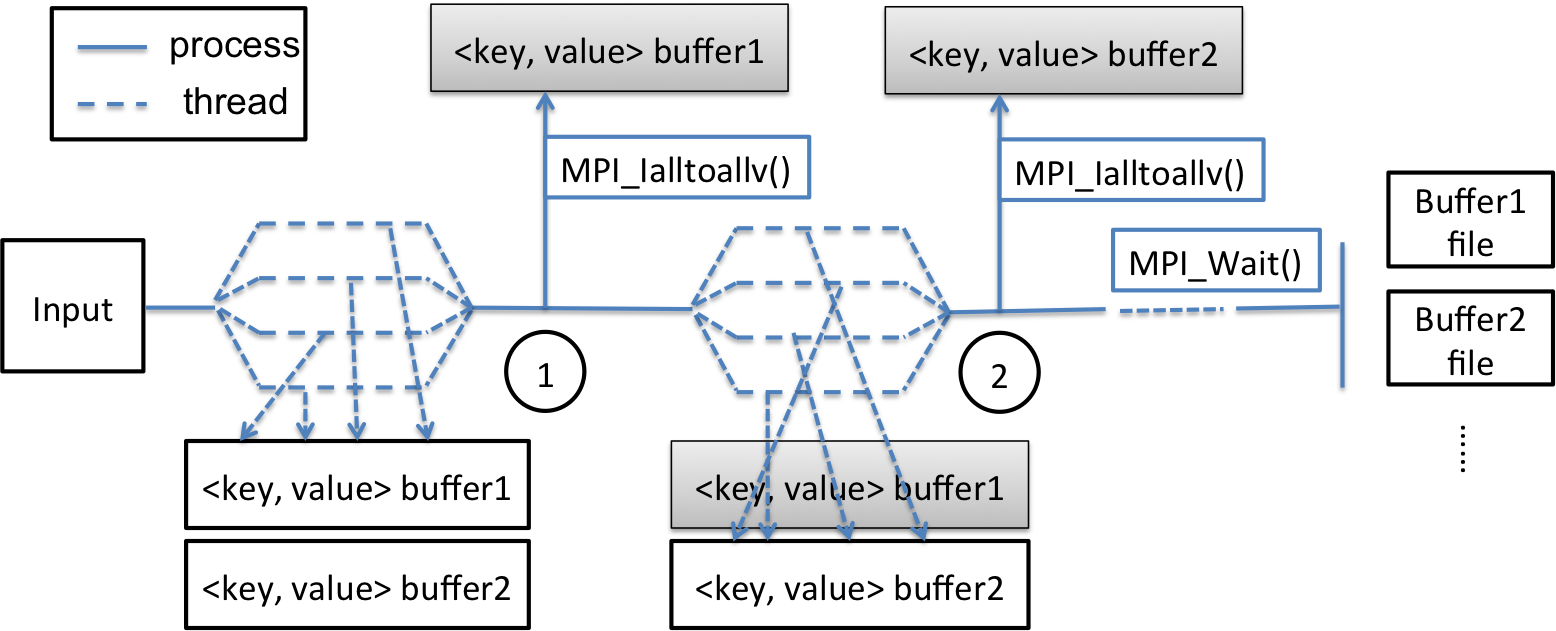
\includegraphics[width=0.8\linewidth,height=2.2in]{figs/multithreaded_map_design.png}
  \caption{Design of multithreaded Map phase.}
  \label{fig:multithreaded_map}
\end{figure*}

The key idea of the design is to use one process on each node to ensure
node to node communication (instead of multiple communication channels
among two nodes), and to use multiple threads to apply the map function
to generate the intermediate key value pairs. To enable the design, we 
use two buffers (double buffer, overflow buffer?) to hold intermediate 
key value pairs for the direct communication among processes (nodes), without
spilling on disk file (which is the case of MR-MPI).

In the map function, the process first reads the input
file into the memory buffer \textit{in\_buffer}, (called \textit{in\_buffer}, size is configureable 
by the user). At the same time, each process
maintains two memory buffers (named \textit{kv\_buffer1} and \textit{kv\_buffer2}) 
to store the intermediate output of map function. After the \textit{in\_buffer} is
populated with data records, the program spawns an OpenMP parallel
session, in which each thread reads a distinct part of the data records
in \textit{in\_buffer}, applies the user defined map function, and writes the
intermediate output to the \textit{kv\_buffer} collectively. When the 
\textit{kv\_buffer} is full, it is used as the MPI send buffer in the non-blocking
MPI\_Ialltoallv communication to send key value pairs. 

\subsection{Multithreaded reduce}

Key point:
\begin{itemize}
\item almost entirely multithreaded
\item use dictionary and hash table to reorganize 
\end{itemize}

The use of dictionary and hash table are suggested by yanfei, need to point out.








\section{Evaluation}
\label{s:evaluation}

\subsection{Platform and benchmarks}


\subsection{Performance results }





\section{Related work}
\label{s:related_work}

\section{Conclusion and future work}
\label{s:conclusions}

In this paper, we presented a method to study intra- and
inter-trajectory analysis in large protein-folding datasets on
distributed memory systems. Our method is a one-pass, distributed
process that is efficient and suitable for in-situ data analysis:
it avoids the need for moving trajectory data, uses a limited amount of 
memory, and is faster than traditional approaches.
We implemented the method in a modular framework using
Parallel MATLAB and evaluated its performance using the folding
trajectory of the protein HP-35 NleNle (i.e., a variant of the villin
headpiece subdomain) on 256 compute cores of Gordon supercomputer. 
We compared our method's performance with a more traditionally used,
centralized approach and observed significantly faster runtimes
(i.e., two orders of magnitude faster, 41.5 seconds comparing to 3
hours in the traditional method). We also observed a three and four
orders of magnitude reduction respectively in the size of data
movement and memory usage (i.e., 6.9 MB memory usage comparing to 16
GB in the traditional method, 4.4 KB data moved comparing to 539
MB). In addition, our method presents a linear weak scalability and
maintains a parallel efficiency above 90\% when using up to 128
cores. 

Future work includes testing the accuracy and scalability of our method for 
larger datasets of protein-folding trajectories containing more diverse
protein conformations (i.e., alpha-helix and beta-sheet) than the
villin subdomain and for larger distributed memory systems. We are also 
committed to closely work with domain scientists to
explore the benefit of our method to the study of the protein-folding
process.

\balance


% use section* for acknowledgement
\section*{Acknowledgment}
This work is supported in part by NSF grants: DMS 0800272/0800266, and CCF-SHF 1318445/1318417. This work used the Extreme Science and Engineering Discovery Environment (XSEDE), which is supported by National Science Foundation grant number OCI-1053575. The authors want to thank Dr. Vijay Pande and T. J. Lane from Stanford  for providing us with the dataset for our tests. All the software will be made available before the conference. 

%\newpage
% trigger a \newpage just before the given reference
% number - used to balance the columns on the last page
% adjust value as needed - may need to be readjusted if
% the document is modified later
%\IEEEtriggeratref{8}
% The "triggered" command can be changed if desired:
%\IEEEtriggercmd{\enlargethispage{-5in}}

% references section

% can use a bibliography generated by BibTeX as a .bbl file
% BibTeX documentation can be easily obtained at:
% http://www.ctan.org/tex-archive/biblio/bibtex/contrib/doc/
% The IEEEtran BibTeX style support page is at:
% http://www.michaelshell.org/tex/ieeetran/bibtex/
%\bibliographystyle{IEEEtran}
% argument is your BibTeX string definitions and bibliography database(s)
%\bibliography{paper}
%
% <OR> manually copy in the resultant .bbl file
% set second argument of \begin to the number of references
% (used to reserve space for the reference number labels box)
%\begin{thebibliography}{11}
%
%\bibitem{IEEEhowto:kopka}
%H.~Kopka and P.~W. Daly, \emph{A Guide to \LaTeX}, 3rd~ed.\hskip 1em plus
%  0.5em minus 0.4em\relax Harlow, England: Addison-Wesley, 1999.
%
%\end{thebibliography}

% Generated by tran.bst, version: 1.13 (2008/09/30)
%\small
\begin{thebibliography}{10}
%\providecommand{\url}[1]{#1}
%\csname url@samestyle\endcsname
%\providecommand{\newblock}{\relax}
%\providecommand{\bibinfo}[2]{#2}
%\providecommand{\BIBentrySTDinterwordspacing}{\spaceskip=0pt\relax}
%\providecommand{\BIBentryALTinterwordstretchfactor}{4}
%\providecommand{\BIBentryALTinterwordspacing}{\spaceskip=\fontdimen2\font plus
%\BIBentryALTinterwordstretchfactor\fontdimen3\font minus
%  \fontdimen4\font\relax}
%\providecommand{\BIBforeignlanguage}[2]{{%
%\expandafter\ifx\csname l@#1\endcsname\relax
%\typeout{** WARNING: tran.bst: No hyphenation pattern has been}%
%\typeout{** loaded for the language `#1'. Using the pattern for}%
%\typeout{** the default language instead.}%
%\else
%\language=\csname l@#1\endcsname
%\fi
%#2}}
%\providecommand{\BIBdecl}{\relax}
%\BIBdecl

\bibitem{Phillips2011} J.~Phillips et al., ``Validating clustering of
  molecular dynamics simulations using polymer models,'' \emph{BMC
    Bioinformatics}, vol.~12, no.~1, pp. 445--467, 2011.  
\bibitem{Tu2008} T.~Tu et al., ``A scalable parallel framework for
  analyzing terascale molecular dynamics simulation trajectories,'' in
  \emph{Proc. of the 2008 ACM/IEEE International Conference for High
    Performance Computing, Networking, Storage and Analysis (SC'08)}, pp. 1--12, 2008.
\bibitem{Best2002} C.~Best and H.~C. Hege, ``Visualizing and
  identifying conformational ensembles in molecular dynamics
  trajectories,'' \emph{Computing in Science Engineering}, vol.~4,
  no.~3, pp. 68--75, 2002.
\bibitem{bigdataweb} M. Stonebraker. (2012, Sept. 21). What does big
  data mean [ONLINE]. Available:
  http://cacm.acm.org/blogs/blog-cacm/155468-what-does-big-data-mean/fulltext
\bibitem{Bennett2012} J.~C. Bennett et al., ``Combining in-situ and
  in-transit processing to enable extreme-scale scientific analysis,''
  in \emph{Proc. of the 2012 ACM/IEEE International Conference for
    High Performance Computing, Networking, Storage and Analysis
    (SC'12)}, pp. 1--9, 2012.
\bibitem{Lakshminarasimhan2013} S.~Lakshminarasimhan et al.,
  ``Scalable in-situ scientific data encoding for analytical query
  processing,'' in \emph{Proc. of the 22nd International Symposium on
    High-performance Parallel and Distributed Computing (HPDC '13)}, pp. 1--12, 2013.
\bibitem{Cordeiro2011} R.~L.~F. Cordeiro et al., ``Clustering very
  large multi-dimensional datasets with {MapReduce},'' in
  \emph{Proc. of the 17th ACM SIGKDD International Conference on
    Knowledge Discovery and Data Mining (KDD'11)}, pp. 690--698, 2011.
\bibitem{Liu2013} J.~Liu et al., ``Segmented analysis for reducing
  data movement,'' in \emph{Proc. of the IEEE International conference
    on Big Data (BigData'13)}, 2013.
\bibitem{Pande2007} D.~L. Ensign et al., ``Heterogeneity even at the
  speed limit of folding: large-scale molecular dynamics study of a
  fast-folding variant of the villin headpiece,'' \emph{Journal of
    Molecular Biology}, vol.  374, no.~3, pp. 806--816, 2007.
\bibitem{Borg2009} I.~Borg and P.~J.~F. Groenen, \emph{Modern
  multidimensional scaling: theory and applications}, Springer, 2005.
\bibitem{FCM} R.~L. Cannon et al., ``Efficient implementation of the
  fuzzy c-means clustering algorithms,'' \emph{IEEE Transactions on
    Pattern Analysis and Machine Intelligence}, vol.~8, no.~2,
  pp. 248--255, 1986. 
    \bibitem{Mooi2011} E.~Mooi and M.~Sarstedt, ``Chapter 9 -
      clustering analysis", in \emph{A Concise Guide to Market
        Research: The Process, Data, and Methods Using {IBM} {Spss}
        Statistics}, Springer, 2011.  
\bibitem{pearson} G.~W. Snedecor and W.~G. Cochran, ``The sample
  correlation coefficient {R}", in \emph{Statistical Methods}, 7th
  ed. Iowa State Press,1980.
  \bibitem{Moler1995} C.~Moler, ``Why there isn't parallel {MATLAB},''
    \emph{Mathworks Newsletter}, vol.~00, pp. 1--12, 1995.
\bibitem{Moler2013} C. Moler, ``Parallel {MATLAB}: {from hell no to
  you bet},'' \emph{Thirty Years of Parallel Computing at Argonne: A
  Symposium}, May 2013.
\end{thebibliography}

%[Total times in seconds across processes broken down into distinctive components: Map (M), Shuffle (S), Overhead (O), Reduce (R), and Total (T).]
%This is the appendix.


% that's all folks
\end{document}



% LocalWords:  priori
